\documentclass{tufte-book}
%\documentclass[twoside,symmetric]{tufte-book}
\hypersetup{colorlinks}% uncomment this line if you prefer colored hyperlinks (e.g., for onscreen viewing)

%%
% Book metadata
\title{Introduction \\to Python \thanks{Thanks to Edward R.~Tufte for his inspiration.}}
\author[The Tufte-LaTeX Developers]{CSEF}
\publisher{The Student Academy}

%%
% If they're installed, use Bergamo and Chantilly from www.fontsite.com.
% They're clones of Bembo and Gill Sans, respectively.
%\IfFileExists{bergamo.sty}{\usepackage[osf]{bergamo}}{}% Bembo
%\IfFileExists{chantill.sty}{\usepackage{chantill}}{}% Gill Sans

%\usepackage{microtype}

%%
% Just some sample text
\usepackage{lipsum}

%%
% For nicely typeset tabular material
\usepackage{booktabs}

%%
% For graphics / images
\usepackage{graphicx}
\setkeys{Gin}{width=\linewidth,totalheight=\textheight,keepaspectratio}
\graphicspath{{graphics/}}

%%
% Additional
\usepackage{units}
\usepackage{amsmath,amsfonts,amsthm} % Math packages
\usepackage{mathtools}% http://ctan.org/pkg/mathtools
%\usepackage{mparhack}
\usepackage{sectsty} % Allows customizing section commands
\usepackage[dvipsnames]{xcolor}
\usepackage{pgf,tikz}
\usepackage{pgfplots}
\usetikzlibrary{shapes,arrows}
\usetikzlibrary{patterns,fadings}
\usetikzlibrary{arrows}
 \usetikzlibrary{decorations.pathreplacing}
 \usetikzlibrary{snakes}
 \usetikzlibrary{spy}
 \usepackage{setspace}
% \usepackage{3dplot}
 \usepackage{cancel}
%\usepackage{physymb}
\usepackage{braket}
\usepackage{verbatim}
%\usepackage[x11names]{xcolor}                     %Additional colors
%\usepackage{euler}  
\usepackage{framed}




% The fancyvrb package lets us customize the formatting of verbatim
% environments.  We use a slightly smaller font.
\usepackage{fancyvrb}
\fvset{fontsize=\normalsize}

%%
% Prints argument within hanging parentheses (i.e., parentheses that take
% up no horizontal space).  Useful in tabular environments.
\newcommand{\hangp}[1]{\makebox[0pt][r]{(}#1\makebox[0pt][l]{)}}

%%
% Prints an asterisk that takes up no horizontal space.
% Useful in tabular environments.
\newcommand{\hangstar}{\makebox[0pt][l]{*}}

%%
% Prints a trailing space in a smart way.
\usepackage{xspace}




% Prints the month name (e.g., January) and the year (e.g., 2008)
\newcommand{\monthyear}{%
  \ifcase\month\or January\or February\or March\or April\or May\or June\or
  July\or August\or September\or October\or November\or
  December\fi\space\number\year
}


% Prints an epigraph and speaker in sans serif, all-caps type.
\newcommand{\openepigraph}[2]{%
  %\sffamily\fontsize{14}{16}\selectfont
  \begin{fullwidth}
  \sffamily\large
  \begin{doublespace}
  \noindent\allcaps{#1}\\% epigraph
  \noindent\allcaps{#2}% author
  \end{doublespace}
  \end{fullwidth}
}

% Inserts a blank page
\newcommand{\blankpage}{\newpage\hbox{}\thispagestyle{empty}\newpage}

\usepackage{units}

% Typesets the font size, leading, and measure in the form of 10/12x26 pc.
\newcommand{\measure}[3]{#1/#2$\times$\unit[#3]{pc}}

% Macros for typesetting the documentation
\newcommand{\hlred}[1]{\textcolor{Maroon}{#1}}% prints in red
\newcommand{\hangleft}[1]{\makebox[0pt][r]{#1}}
\newcommand{\hairsp}{\hspace{1pt}}% hair space
\newcommand{\hquad}{\hskip0.5em\relax}% half quad space
\newcommand{\TODO}{\textcolor{red}{\bf TODO!}\xspace}
\newcommand{\ie}{\textit{i.\hairsp{}e.}\xspace}
\newcommand{\eg}{\textit{e.\hairsp{}g.}\xspace}
\newcommand{\na}{\quad--}% used in tables for N/A cells
\providecommand{\XeLaTeX}{X\lower.5ex\hbox{\kern-0.15em\reflectbox{E}}\kern-0.1em\LaTeX}
\newcommand{\tXeLaTeX}{\XeLaTeX\index{XeLaTeX@\protect\XeLaTeX}}
% \index{\texttt{\textbackslash xyz}@\hangleft{\texttt{\textbackslash}}\texttt{xyz}}
\newcommand{\tuftebs}{\symbol{'134}}% a backslash in tt type in OT1/T1
\newcommand{\doccmdnoindex}[2][]{\texttt{\tuftebs#2}}% command name -- adds backslash automatically (and doesn't add cmd to the index)
\newcommand{\doccmddef}[2][]{%
  \hlred{\texttt{\tuftebs#2}}\label{cmd:#2}%
  \ifthenelse{\isempty{#1}}%
    {% add the command to the index
      \index{#2 command@\protect\hangleft{\texttt{\tuftebs}}\texttt{#2}}% command name
    }%
    {% add the command and package to the index
      \index{#2 command@\protect\hangleft{\texttt{\tuftebs}}\texttt{#2} (\texttt{#1} package)}% command name
      \index{#1 package@\texttt{#1} package}\index{packages!#1@\texttt{#1}}% package name
    }%
}% command name -- adds backslash automatically
\newcommand{\doccmd}[2][]{%
  \texttt{\tuftebs#2}%
  \ifthenelse{\isempty{#1}}%
    {% add the command to the index
      \index{#2 command@\protect\hangleft{\texttt{\tuftebs}}\texttt{#2}}% command name
    }%
    {% add the command and package to the index
      \index{#2 command@\protect\hangleft{\texttt{\tuftebs}}\texttt{#2} (\texttt{#1} package)}% command name
      \index{#1 package@\texttt{#1} package}\index{packages!#1@\texttt{#1}}% package name
    }%
}% command name -- adds backslash automatically
\newcommand{\docopt}[1]{\ensuremath{\langle}\textrm{\textit{#1}}\ensuremath{\rangle}}% optional command argument
\newcommand{\docarg}[1]{\textrm{\textit{#1}}}% (required) command argument
\newenvironment{docspec}{\begin{quotation}\ttfamily\parskip0pt\parindent0pt\ignorespaces}{\end{quotation}}% command specification environment
\newcommand{\docenv}[1]{\texttt{#1}\index{#1 environment@\texttt{#1} environment}\index{environments!#1@\texttt{#1}}}% environment name
\newcommand{\docenvdef}[1]{\hlred{\texttt{#1}}\label{env:#1}\index{#1 environment@\texttt{#1} environment}\index{environments!#1@\texttt{#1}}}% environment name
\newcommand{\docpkg}[1]{\texttt{#1}\index{#1 package@\texttt{#1} package}\index{packages!#1@\texttt{#1}}}% package name
\newcommand{\doccls}[1]{\texttt{#1}}% document class name
\newcommand{\docclsopt}[1]{\texttt{#1}\index{#1 class option@\texttt{#1} class option}\index{class options!#1@\texttt{#1}}}% document class option name
\newcommand{\docclsoptdef}[1]{\hlred{\texttt{#1}}\label{clsopt:#1}\index{#1 class option@\texttt{#1} class option}\index{class options!#1@\texttt{#1}}}% document class option name defined
\newcommand{\docmsg}[2]{\bigskip\begin{fullwidth}\noindent\ttfamily#1\end{fullwidth}\medskip\par\noindent#2}
\newcommand{\docfilehook}[2]{\texttt{#1}\index{file hooks!#2}\index{#1@\texttt{#1}}}
\newcommand{\doccounter}[1]{\texttt{#1}\index{#1 counter@\texttt{#1} counter}}

% Generates the index
\usepackage{makeidx}
\makeindex

\begin{document}

% Front matter
\frontmatter

% r.1 blank page
%\blankpage

% v.2 epigraphs
\newpage\thispagestyle{empty}

\openepigraph{%
The only shibboleth the West has is science. It is the premise of modernity and it defines itself as a rationality capable of, indeed requiring separation from politics, religion and really, society. Modernisation is to work towards this.
}{Bruno Latour}
\vfill
\openepigraph{%
The boundary between science fiction and social reality is an optical illusion.
}{Donna Haraway}


% r.3 full title page
\maketitle




% r.5 contents
\tableofcontents

\listoffigures

\listoftables

% r.7 dedication
\cleardoublepage
~\vfill
\begin{doublespace}
\noindent\fontsize{18}{22}\selectfont\itshape
\nohyphenation
The longest snake ever held captive is Medusa, a reticulated python (python reticulatus). On 12 October 2011, she was measured at 7.67 m long.% \mbox{Edward R.~Tufte} 
%and \mbox{Donald E.~Knuth}.
\end{doublespace}
\vfill
\vfill


% r.9 introduction
%\cleardoublepage
\chapter*{Note}

This physics text is an OpenSource academic project developed in abstraction at The Academy.  The manuscript is written in \LaTeX \ and makes use of the \doccls{tufte-book} and \doccls{tufte-handout} document classes.  

\vspace{2cm}

http://latex-project.org/ftp.html

https://git-scm.com/downloads

%%
% Start the main matter (normal chapters)
\mainmatter

%ints and floats
%\chapter{Boolean}

\section{Intro}

boolean boolean

\section{Boolean Operators}

\section{Boolean Arithmetic}
%\include{rotational_kinematics}
%\include{forces}
%\include{work} 
%\include{momentum} 
%\include{angular_momentum} 
\definecolor{shadecolor}{rgb}{0.9,0.9,0.9}











\chapter{While Loops}

A {\color{red}while loop} statement in Python programming language repeatedly executes a target statement as long as a given condition is true.

\vspace{1cm}
The condition may be any expression, and true is any non-zero value. The loop iterates while the condition is true.When the condition becomes false, program control passes to the line immediately following the loop.In Python, all the statements indented by the same number of character spaces after a programming construct are considered to be part of a single block of code. Python uses indentation as its method of grouping statements.

\begin{marginfigure}
  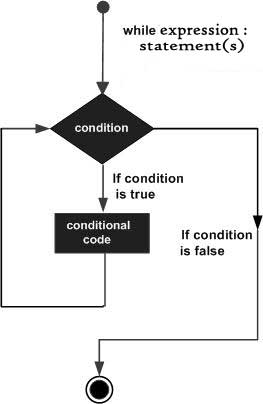
\includegraphics[width=\linewidth]{whileloop.jpeg}
  \caption{Flow diagram about how the while loop works}
  \label{fig:marginfig}
\end{marginfigure}

\vspace{0.5cm}
\subsection{Python code example}
\begin{framed}
\begin{verbatim}

count = 0
while (count < 9):
   print 'The count is:', count
   count = count + 1

print "Good bye!"

\end{verbatim}
\end{framed}

\subsection{Output}
\marginnote[40pt]{The code will produce the following output.}
\begin{shaded}
\begin{verbatim}
>>> 
The count is: 0
The count is: 1
The count is: 2
The count is: 3
The count is: 4
The count is: 5
The count is: 6
The count is: 7
The count is: 8
Good bye!
>>> 
\end{verbatim}
\end{shaded}

\subsection{Infinite Loop}
A loop becomes {\color{red}infinite loop} if a condition never becomes {\textbf{FALSE}}. You must use caution when using while loops because of the possibility that this condition never resolves to a FALSE value. This results in a loop that never ends. Such a loop is called an infinite loop.

An infinite loop might be useful in client/server programming where the server needs to run continuously so that client programs can communicate with it as and when required.
\marginnote[40pt]{This python code is an example of how infinite loop can be created.}
\begin{framed}
\begin{verbatim}
var = 1
while var == 1:
   num = raw_input("Enter a number  :")
   print "You entered: ", num

print "Good bye!"
\end{verbatim}
\end{framed}

\marginnote[40pt]{This code creates an infinite loop where it will need your input of any number.Once you input any number, it will output it like if you input "X" it will show back "X".}
\begin{shaded}
\begin{verbatim}

Enter a number  :X
You entered:  x
Enter a number  :Y
You entered:  Y
Enter a number  :Z
You entered:  Z
Enter a number between :

\end{verbatim}
\end{shaded}

To break the loop you will either need to add the "{\color{red}break}" command in your code OR press {\textbf{CTRL+C} to exit the program.

\subsection{Using else statements with while loops}
Python supports to have an else statement associated with a loop statement.

If the {\color{red}else statement} is used with a while loop, the else statement is executed when the condition becomes false.

\vspace{1cm}







\begin{framed}
\begin{verbatim}

count = 0
while count < 5:
   print count, " is  less than 5"
   count = count + 1
else:
   print count, " is not less than 5"

\end{verbatim}
\end{framed}

\marginnote[-140pt]{The following code illustrates the combination of an else statement with a while statement that prints a number as long as it is less than 5, otherwise else statement gets executed.}

\marginnote[40pt]{This is the output in python when the code above is executed.}
\begin{shaded}
\begin{verbatim}
>>> 
0 is less than 5
1 is less than 5
2 is less than 5
3 is less than 5
4 is less than 5
5 is not less than 5
>>> 
\end{verbatim}
\end{shaded}










%\bibliography{sample-handout}
%\bibliographystyle{plainnat}


\printindex

\end{document}

